\section{Register Module}

\begin{figure}[h!]
    \centering
    \vspace{1em}
\scalebox{0.85}{
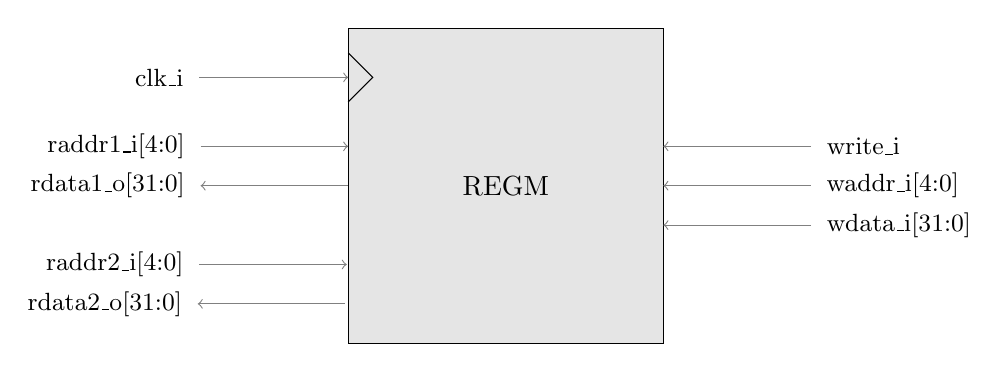
\begin{tikzpicture}[scale=1.25, draw=gray, inner sep=0, outer sep=0]
  \node[rectangle, draw=black,
    align=center,
    minimum height = 4cm,
    minimum width = 4cm,
    fill = gray!20] (block) at (0, 0) {REGM};

  \node (lport2) at ([yshift=0cm]block.west) {};
  \node (lport1) at ([yshift=0.4cm]lport2.center) {};
  \draw[->] ([xshift=-1.5cm]lport1.center) node[left=0.2cm, anchor=east]{\small raddr1\_i[4:0]} -- (lport1.center);
  \draw[<-] ([xshift=-1.5cm]lport2.center) node[left=0.2cm, anchor=east]{\small rdata1\_o[31:0]} -- (lport2.center);

  \node (lport3) at ([yshift=-0.8cm]lport2.west) {};
  \node (lport4) at ([yshift=-0.4cm]lport3.west) {};
  \draw[->] ([xshift=-1.5cm]lport3.center) node[left=0.2cm, anchor=east]{\small raddr2\_i[4:0]} -- (lport3.center);
  \draw[<-] ([xshift=-1.5cm]lport4.center) node[left=0.2cm, anchor=east]{\small rdata2\_o[31:0]} -- (lport4.center);

  \node (rport2) at (block.east) {};
  \node (rport1) at ([yshift=0.4cm]rport2.center) {};
  \node (rport3) at ([yshift=-0.4cm]rport2.center) {};
  \draw[->] ([xshift=1.5cm]rport1.center) node[right=0.2cm, anchor=west]{\small write\_i} -- (rport1.center);
  \draw[->] ([xshift=1.5cm]rport2.center) node[right=0.2cm, anchor=west]{\small waddr\_i[4:0]} -- (rport2.center);
  \draw[->] ([xshift=1.5cm]rport3.center) node[right=0.2cm, anchor=west]{\small wdata\_i[31:0]} -- (rport3.center);

  \node (clk) at ([yshift=-0.5cm]block.north west) {};
  \draw[->] ([xshift=-1.5cm]lport3.center |- clk.center) node[left=0.2cm, anchor=east]{\small clk\_i} -- (clk.center);
  % clk triangle
  \draw[-, draw=black] ([yshift=0.25cm]clk.center) -- ([xshift=0.25cm]clk.center) -- ([yshift=-0.25cm]clk.center);
\end{tikzpicture}
}

    \caption{Schematic view of the Register Module}
    \label{fig:regm}
\end{figure}

\subsection{Interface}

\begin{content}
The register module implements the 32 internal registers of ECAP5-DPROC. It has two reading port and one writing port. The signals are described in table \ref{tab:regm-interface}. 
\end{content}

{
  \vspace{0.5em}
  \begin{center}
    \refstepcounter{table}
    Table \thetable: Register Module interface signals\label{tab:regm-interface}
  \end{center}

\footnotesize
\begin{xltabular}{0.9\textwidth}{|l|c|c|X|}
  \hline
  \cellcolor{gray!20}\textbf{NAME} & \cellcolor{gray!20}\textbf{TYPE} & \cellcolor{gray!20}\textbf{WIDTH} & \cellcolor{gray!20}\textbf{DESCRIPTION} \\
  \hline
  clk\_i & I & 1 & Clock input. \\
  \hline
  \multicolumn{4}{|l|}{\textbf{FIRST READING PORT}} \\
  \hline
  raddr1\_i & I & 5 & Register selector. \\
  \hline
  rdata1\_o & O & 32 & Selected register value. \\
  \hline
  \multicolumn{4}{|l|}{\textbf{SECOND READING PORT}} \\
  \hline
  raddr2\_i & I & 5 & Register selector. \\
  \hline
  rdata2\_o & O & 32 & Selected register value. \\
  \hline
  \multicolumn{4}{|l|}{\textbf{WRITING PORT}} \\
  \hline
  waddr\_i & I & 5 & Register selector. \\
  \hline
  write\_i & I & 1 & Asserted to indicate a write. \\
  \hline
  wdata\_i & I & 32 & Data to be written. \\
  \hline
\end{xltabular}
}


\subsection{Specification}

\subsubsection{Upstream requirements}

The table \ref{tab:regm-upstream-requirements} outlines the upstream requirements applicable to the Register Module.

{
  \vspace{0.5em}
  \begin{center}
    \refstepcounter{table}
    Table \thetable: Upstream requirements applicable to the External Memory Module\label{tab:regm-upstream-requirements}
  \end{center}
  
\footnotesize
\begin{xltabular}{0.9\textwidth}{|X|c|}
  \hline
  \cellcolor{gray!20}\textbf{ID} \\
  \hline
  F\_REGISTERS\_01 \\
  \hline
  F\_REGISTERS\_02 \\
  \hline
\end{xltabular}
}


\subsubsection{Functional requirements}

\req{D\_REGM\_REGISTERS\_01}{
  The register module shall implement 32 general purpose registers ranging from \texttt{x0} to \texttt{x31}.
}[
  derivedfrom=F\_REGISTERS\_01
]

\req{D\_REGM\_READ\_PORT\_01}{
  The \texttt{rdata1\_o} signal shall be set asynchronously to the value of the register pointed by \texttt{raddr1\_i}.
}[
  derivedfrom=F\_REGISTERS\_01
]

\req{D\_REGM\_READ\_PORT\_02}{
  The \texttt{rdata2\_o} signal shall be set asynchronously to the value of the register pointed by \texttt{raddr2\_i}.
}[
  derivedfrom=F\_REGISTERS\_01
]

\req{D\_REGM\_WRITE\_PORT\_01}{
  The value of the register pointed by \texttt{waddr\_i} shall be set to \texttt{wdata\_i} on the rising edge of \texttt{clk\_i} when \texttt{write\_i} is asserted.
}[
  derivedfrom=F\_REGISTERS\_01
]

\req{D\_REGM\_WRITE\_PORT\_02}{
  When both reading and writing to the same registers, the read operation shall be performed before the write operation.
}[
  derivedfrom=F\_REGISTERS\_01
]

\req{D\_REGM\_WRITE\_PORT\_03}{
  The value of register \texttt{x0} shall not be changed during a write operation, remaining the constant zero.
}[
  derivedfrom=F\_REGISTERS\_02
]

\subsection{Behavior}

\subsubsection{Read behavior}

\begin{content}
  When reading, \texttt{rdata1\_i} and \texttt{rdata2\_i} output, on the rising edge of \texttt{clk\_i}, the value of the register respectively selected by \texttt{raddr1\_i}
and \texttt{raddr2\_i}.
\end{content}

\begin{figure}[H]
    \centering
    \makeatletter\gdef\dividers{}
\begin{tikztimingtable}[%
    scale=0.7,
    timing/dslope=0.1,
    timing/.style={x=5ex,y=3ex},
    x=5ex,
    timing/rowdist=4ex,
    timing/name/.style={font=\footnotesize},
    timing/u/background/.style={fill=gray!20},
    timing/e/background/.style={fill=gray!20},
]
clk\_i & H 6{C C} L \\
& \divider{First read port} \\
raddr1\_i[4:0] &  2U 2D{0x5} 2D{0x2} 2U 2U       2D{0x0} 2U\\
rdata1\_o[31:0] & 2U 2D{x5}  2D{x2}  2U 2U       2D{x0}  2U \\
& \divider{Second read port} \\
raddr2\_i[4:0] &  2U 2D{0x5} 2D{0x6} 2U 2D{0x1F} 2U      2U\\
rdata2\_o[31:0] & 2U 2D{x5}  2D{x6}  2U 2D{x31}  2U      2U \\
\extracode
% grid
\begin{pgfonlayer}{background}
\begin{scope}[semitransparent ,semithick]
\vertlines[darkgray,dotted]{2, 4, 6, 8, 10, 12}
\dividers
\end{scope}
\end{pgfonlayer}
\end{tikztimingtable}

    \caption{Timing diagram of the read behavior of the register module}
    \label{fig:regm-behavior-read}
\end{figure}

\subsubsection{Write behavior}

\begin{content}
A register write happens on the rising edge of \texttt{clk\_i} when \texttt{write\_i} is asserted, writing the value \texttt{wdata\_i} in the register selected by \texttt{wad
r\_i}.
\end{content}

\begin{figure}[H]
    \centering
    \makeatletter\gdef\dividers{}
\begin{tikztimingtable}[%
    scale=0.7,
    timing/dslope=0.1,
    timing/.style={x=5ex,y=3ex},
    x=5ex,
    timing/rowdist=4ex,
    timing/name/.style={font=\footnotesize},
    timing/u/background/.style={fill=gray!20},
    timing/e/background/.style={fill=gray!20},
]
clk\_i & H 7{C C} L \\
& \divider{Write port} \\
write\_i &       2E 2H      2H      2E 2H      2U 2H      2E \\
waddr\_i[4:0] &  2U 2D{0x5} 2D{0x2} 2U 2D{0x0} 2U 2D{0x5} 2U \\
wdata\_i[31:0] & 2U 2D{a}   2D{b}   2U 2D{c}   2U 2D{d}   2U \\
& \divider{Internal register values} \\
x0 & 16D{0x0} \\
x2 & 2U 2.5U 11.5D{b} \\
x5 & 2.5U 10D{a} 3.5D{d} \\
\extracode
% grid
\begin{pgfonlayer}{background}
\begin{scope}[semitransparent ,semithick]
\vertlines[darkgray,dotted]{2, 4, 6, 8, 10, 12, 14}
\dividers
\end{scope}
\end{pgfonlayer}
\end{tikztimingtable}

    \caption{Timing diagram of the write behavior of the register module}
    \label{fig:regm-behavior-write}
\end{figure}

\subsubsection{Read-before-write behavior}

\begin{content}
    When both read and write operations are requested on the same register at the same time, the write operation happens during the next clock cycle. Considering read request
 are performed during the second stage of the pipeline while write requests are performed during the fourth stage, this behavior reduces the potential hazards induces by the pipe
ined architecture.

    Figure \ref{fig:regm-behavior-read-before-write} provides an example with a read request on the first port, although this behavior also applies to the second reading port

\end{content}

\begin{figure}[H]
    \centering
    \makeatletter\gdef\dividers{}
\begin{tikztimingtable}[%
    scale=0.7,
    timing/dslope=0.1,
    timing/.style={x=5ex,y=3ex},
    x=5ex,
    timing/rowdist=4ex,
    timing/name/.style={font=\footnotesize},
    timing/u/background/.style={fill=gray!20},
    timing/e/background/.style={fill=gray!20},
]
clk\_i & H 3{C C} L \\
& \divider{Read port} \\
raddr1\_i[4:0]  & 2U 2D{0x5} 2D{0x5} 2U \\
rdata1\_o[31:0] & 2.5U 2D{x5}  2D{a}   1.5U \\
& \divider{Write port} \\
write\_i        & 2E 2H      2L      2E \\
waddr\_i[4:0]   & 2U 2D{0x5} 2U      2U \\
wdata\_i[31:0]  & 2U 2D{a}   2U      2U \\
& \divider{Internal register value} \\
x5 & 2.5D{x5} 5.5D{a} \\
\extracode
% grid
\begin{pgfonlayer}{background}
\begin{scope}[semitransparent ,semithick]
\vertlines[darkgray,dotted]{2, 4, 6}
\dividers
\end{scope}
\end{pgfonlayer}
\end{tikztimingtable}

    \caption{Timing diagram of the read-before-write behavior of the register module}
    \label{fig:regm-behavior-read-before-write}
\end{figure}

\newpage
